\documentclass[12pt]{letter} % Default font size of the document, change to 10pt to fit more text

\usepackage{tikz}
\usetikzlibrary{shapes.geometric, arrows}



\tikzstyle{normal} = [rectangle, rounded corners, minimum width=3cm, minimum height=1cm, text centered, text width=3.5cm, draw=black, fill=lightgray]

\tikzstyle{invis} = [rectangle, minimum width=1cm, minimum height=1cm, text centered, text width=1cm, draw opacity=1]


%\tikzstyle{startstop} = [rectangle, rounded corners, minimum width=3cm, minimum height=1cm,text centered, text width=5.5cm, draw=black, fill=lightgray]


%\tikzstyle{io} = [trapezium, trapezium left angle=70, trapezium right angle=110, minimum width=3cm, minimum height=1cm, text centered, draw=black, fill=blue!30]

%\tikzstyle{process} = [rectangle, minimum width=3cm, minimum height=1cm, text centered, text width=3cm, draw=black, fill=orange!30]
%\tikzstyle{decision} = [diamond, minimum width=3cm, minimum height=1cm, text centered, draw=black, fill=green!30]

\tikzstyle{arrow} = [thick,->,>=stealth]

\begin{document}


1. Test retest
\vspace{0.57in}

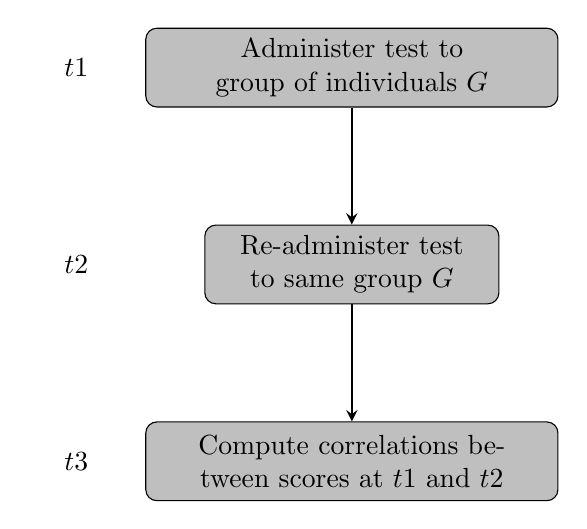
\begin{tikzpicture}[node distance=2.5cm]

%% NODES

\node (t1_label) [invis] {$t1$};
\node (t1) [normal, right of=t1_label, text width=5cm, node distance=3.5cm] {Administer test to group of individuals $G$};
\node (t2_label) [invis, below of=t1_label] {$t2$};
\node (t2) [normal, right of=t2_label, node distance=3.5cm] {Re-administer test to same group $G$};
\node (t3_label) [invis, below of=t2_label] {$t3$};
\node (t3) [normal, right of=t3_label, text width=5cm,node distance=3.5cm] {Compute correlations between scores at $t1$ and $t2$};


%% ARROWS 

\draw [arrow] (t1) -- (t2);
%node[anchor=west] {Time elapsing}
\draw [arrow] (t2) -- (t3);

\end{tikzpicture}


\pagebreak


2. Parallel forms
\vspace{0.57in}

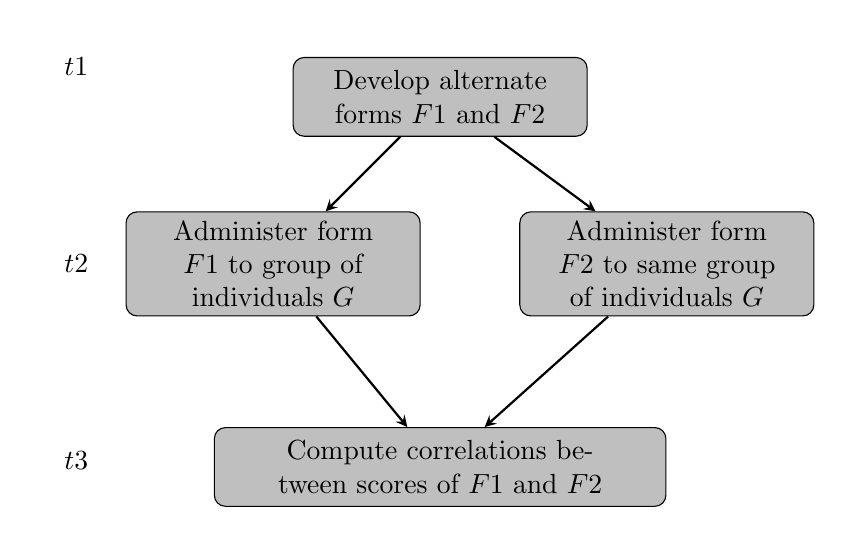
\begin{tikzpicture}[node distance=2.5cm]

%% NODES

\node (t1) [normal] {Develop alternate forms $F1$ and $F2$};
\node (t2a) [normal, below left of=t1, node distance=3cm] {Administer form $F1$ to group of individuals $G$};
\node (t2b) [normal, right of=t2a, node distance=5cm] {Administer form $F2$ to same group of individuals $G$};
\node (t2_label) [left of=t2a] {$t2$};
\node (t1a) [invis, above of=t2a] {};
\node (t1_label) [invis, left of=t1a] {$t1$};
\node (t3) [normal, below of=t1, text width=5.5cm,  node distance=4.7cm] {Compute correlations between scores of $F1$ and $F2$};
\node (t3_label)[invis, below of=t2_label] {$t3$};


%% ARROWS 

\draw [arrow] (t1) -- (t2a);
\draw [arrow] (t1) -- (t2b); 
%node[anchor=west] {Time elapsing}
\draw [arrow] (t2a) -- (t3);
\draw [arrow] (t2b) -- (t3);

\end{tikzpicture}


\pagebreak


3. Split-half
\vspace{0.57in}

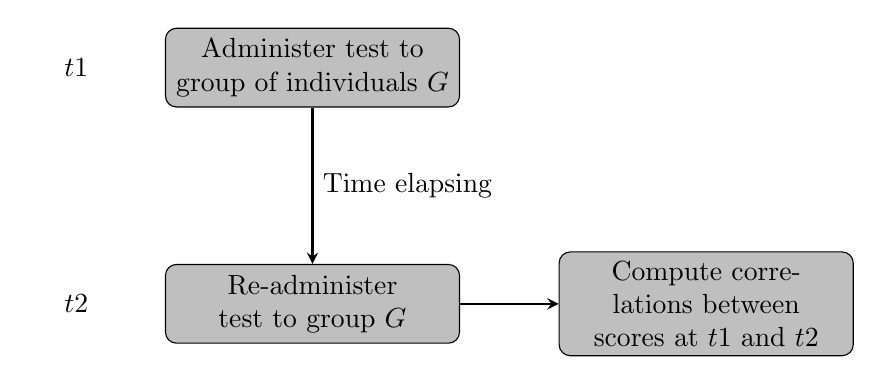
\begin{tikzpicture}[node distance=3cm]

%% NODES

\node (t1_label) [invis] {$t1$};
\node (t1) [normal, right of=t1_label] {Administer test to group of individuals $G$};
\node (t2_label) [invis, below of=t1_label] {$t2$};
\node (t2) [normal, right of=t2_label] {Re-administer test to group $G$};
\node (t3) [normal, right of=t2, node distance=5cm] {Compute correlations between scores at $t1$ and $t2$};


%% ARROWS 

\draw [arrow] (t1) -- node[anchor=west] {Time elapsing} (t2);
\draw [arrow] (t2) -- (t3);

\end{tikzpicture}


\pagebreak


4. Internal consistency
\vspace{0.57in}

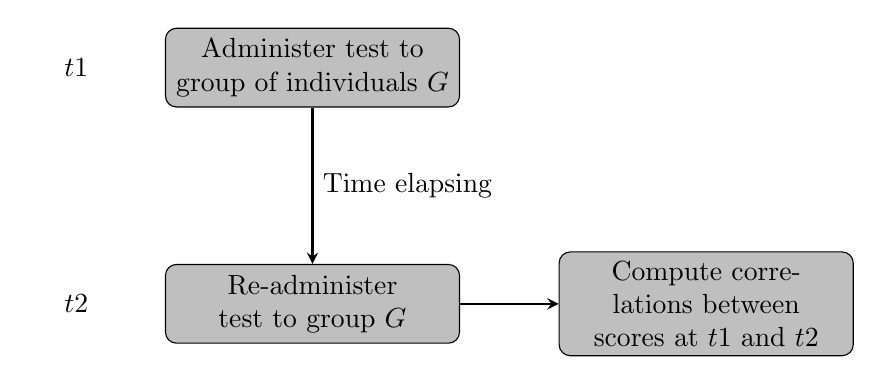
\begin{tikzpicture}[node distance=3cm]

%% NODES

\node (t1_label) [invis] {$t1$};
\node (t1) [normal, right of=t1_label] {Administer test to group of individuals $G$};
\node (t2_label) [invis, below of=t1_label] {$t2$};
\node (t2) [normal, right of=t2_label] {Re-administer test to group $G$};
\node (t3) [normal, right of=t2, node distance=5cm] {Compute correlations between scores at $t1$ and $t2$};


%% ARROWS 

\draw [arrow] (t1) -- node[anchor=west] {Time elapsing} (t2);
\draw [arrow] (t2) -- (t3);

\end{tikzpicture}


\pagebreak


5. Inter-rater
\vspace{0.57in}

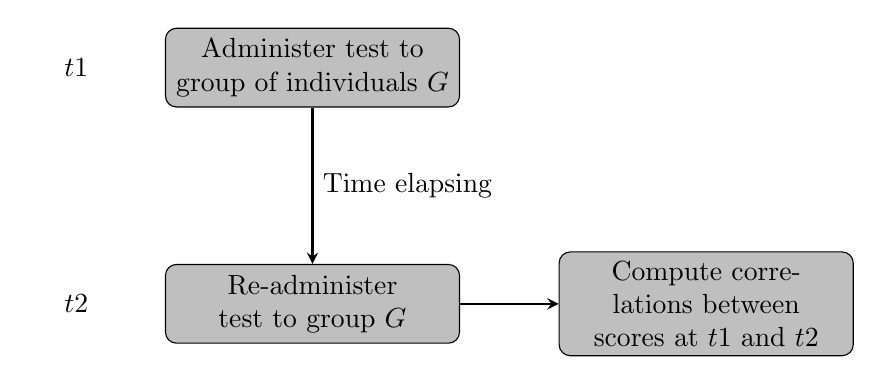
\begin{tikzpicture}[node distance=3cm]

%% NODES

\node (t1_label) [invis] {$t1$};
\node (t1) [normal, right of=t1_label] {Administer test to group of individuals $G$};
\node (t2_label) [invis, below of=t1_label] {$t2$};
\node (t2) [normal, right of=t2_label] {Re-administer test to group $G$};
\node (t3) [normal, right of=t2, node distance=5cm] {Compute correlations between scores at $t1$ and $t2$};


%% ARROWS 

\draw [arrow] (t1) -- node[anchor=west] {Time elapsing} (t2);
\draw [arrow] (t2) -- (t3);

%\draw [arrow] (pro2b) -- (pro1);
%\draw [arrow] (pro2b) |- (pro1);
%\draw [arrow] (pro2a) -- (out1);
%\draw [arrow] (out1) -- (stop);

\end{tikzpicture}


\end{document}